Because of incompressibility, an irrotational flow can be described simply by the \textsc{Laplace} equation
\[
    \nabla^2 \phi = 0 \quad \text{on } \Omega,
\]
such that $\nabla\phi = \uvec$.
We consider the following expression equality.
\[
    \nabla\cdot(\phi_1 \nabla\phi_2 - \phi_2 \nabla\phi_1) = 0.
\]
By the product rule, we have that the left-hand side of the equality is equal to
\[
    \nabla\phi_1 \cdot \nabla\phi_2 + \phi_1 \nabla^2 \phi_2 - \nabla\phi_2 \cdot \nabla\phi_1 + \phi_2 \nabla^2 \phi_1,
\]
which is indeed equal to zero by virtue of the potentials being harmonic.
Considering now the case $\phi_2 = \green$, we may integrate the above equation
\[
    \int_{\Omega} \nabla\cdot(\phi\nabla\green - \green\nabla\phi) \,\dee V = 0,
\]
which by \textsc{Gau\ss}' divergence theorem leads to
\[
    \int_{\partial\Omega} (\phi\partial_n \green - \green \partial_n \phi) \,\dee S = 0.
\]
As will be shown later on in the course, we want to integrate over surfaces where the potential is singular.
The divergence theorem does not hold in such cases, so the singularity must be removed.
This can be remedied by considering a small circle around the singularity situated at $\bzhe$ of radius $\epsilon$.
\begin{figure}[H]
    \centering
    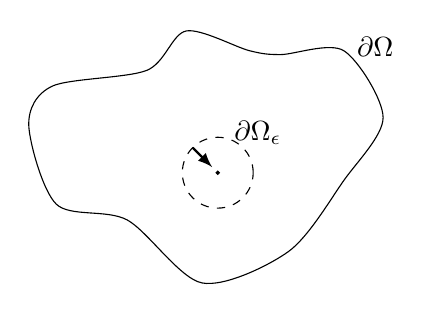
\begin{tikzpicture}
    \begin{scope}[scale = 1]
        \draw plot [smooth cycle] coordinates {(-2, 0) (-1.7, .5) (-.5, .7) (0, 1.2) (.8, .95) (1.2, .9) (2, .95) (2.5, .1) (2, -.7) (1.3, -1.6) (.2, -2) (-.75, -1.2) (-1.65, -1)};
        \draw[dashed] (.4, -.6) circle (.45);
        \draw[fill = black] (.4, -.6) circle (.02) node[below]{$\bzhe$};
        \node at ({.4 + .72*cos(45)}, {-.6 + .72*sin(45)}) {$\partial\Omega_{\epsilon}$};
        \node at (2.4, 1) {$\partial\Omega$};
        \draw[-latex, thick] ({.4 + .45*cos(135)}, {-.6 + .45*sin(135)})--({.4 + .1*cos(135)}, {-.6 + .1*sin(135)});
        \node at ({.4 + .7*cos(135)}, {-.6 + .7*sin(135)}) {$\nhat$};
    \end{scope}
\end{tikzpicture}
\end{figure}

\noindent We may then integrate about this contour to account for the singularity, and ensuring the divergence theorem holds.
\[
    \int_{\partial\Omega_{\epsilon}} (\phi \partial_n \green - \green \partial_n \phi) \,\dee S, \quad \nhat = -\frac{\xvec}{r}.
\]
In two dimensions, the \textsc{Green} function is the logarithm, and we calculate that $\partial_n \ln{r} = -\epsilon^{-1}$.
The differential line element may be discretized as $\dee S = \epsilon \dee\theta$, and for the limiting case of an evanescent $\epsilon$, we may approximate the potential by its \textsc{Taylor} expansion as follows.
\[
    \phi(\xvec) = \phi(\bzhe) + (\xvec - \bzhe)\cdot\nabla\phi(\bzhe) + \cdots = \phi(\bzhe) + O(\epsilon),
\]
since we know $\xvec - \bzhe \leq \epsilon$.
The above integral is then approximated to the first order by
\[
    -\int_{0}^{2\pi} (\phi(\bzhe) + \epsilon \ln{\epsilon} \partial_n \phi) \,\dee\theta,
\]
for which we may consider the limiting case, yielding
\[
    \int_{\partial\Omega_{\epsilon}} (\phi \partial_n \green - \green \partial_n \phi) \,\dee S \approx -2\pi\phi(\bzhe).
\]
Then to the first order, we have in general that for areas of integration enclosing a singularity,
\[
    \int_{\partial\Omega} (\phi \partial_n \green - \green \partial_n \phi) \,\dee S = 2\pi\phi(\bzhe).
\]
Should the singularity lie on the boundary, the integration path is a semicircle.
\begin{figure}[H]
    \centering
    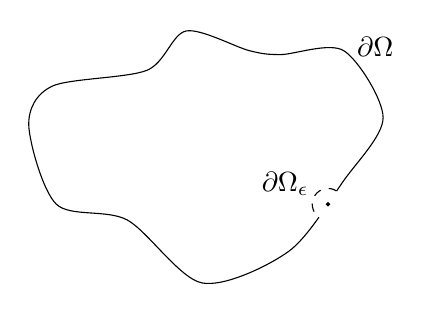
\begin{tikzpicture}
    \begin{scope}[scale = 1]
        %\draw[step = .05] (-2.5,-2) grid (2.5,2);
        \draw plot [smooth cycle] coordinates {(-2, 0) (-1.7, .5) (-.5, .7) (0, 1.2) (.8, .95) (1.2, .9) (2, .95) (2.5, .1) (2, -.7) (1.3, -1.6) (.2, -2) (-.75, -1.2) (-1.65, -1)};
        \node at (2.4, 1) {$\partial\Omega$};
        \def\initialangle{57} \def\endangle{235}
        \def\Ox{1.8} \def\Oy{-1}
        \coordinate (O) at (\Ox, \Oy);
        \draw[very thick, color = white] (O)--({\Ox + .2*cos(\initialangle)}, {\Oy + .2*sin(\initialangle)});
        \draw[very thick, color = white] (O)--({\Ox + .2*cos(\endangle)}, {\Oy + .2*sin(\endangle)});
        \draw[dashed] ({\Ox + .2*cos(\initialangle)}, {\Oy + .2*sin(\initialangle)}) arc (\initialangle:\endangle:.2);
        \draw[fill = black] (O) circle (.02) node[below right]{$\bzhe$};
        \node at ({\Ox + .6*cos(155)}, {\Oy + .6*sin(155)}) {$\partial\Omega_{\epsilon}$}; 
    \end{scope}
\end{tikzpicture}
\end{figure}

\noindent When the singularity is at the boundary like this, the resulting contribution to the integral is consequently halved:
\[
    \int_{\partial\Omega} (\phi \partial_n \green - \green \partial_n \phi) \,\dee S = \pi\phi(\bzhe).
\]
When the singularity is outside the domain of integration, we have seen that the integral is equal to zero.